% !TeX spellcheck = en_US

\chapter{Extending solution DFAs to task DFAs} \label{ch:3}

Given a solution DFA $A_{sol}$ we have determined the following requirements for generating a task DFA $A_{task}$ in our requirements analysis (see~\ref{ch:1:determined-requirements}):
\begin{itemize}
	\item[->] $L(A_{sol}) = L(A_{task})$
	\item[->] $\mmD(A_{sol}) = \mmD(A_{task})$
	\item[->] number of redundant states
	\item[->] number of unreachable states
	\item[->] alphabet size
	\item[->] planarity (can be checked in $O(|Q_{task}|)$)
	\item[->] completeness (for \CompDist-algorithm to work)
\end{itemize}
In order to fulfill these requirements when adding new elements to the given minimal automaton $A_{sol}$, we simply look at how redundant and unreachable states are removed by the minimization algorithm, such that we can deduce from their properties, which restrictions are given for adding such elements. We will show for both classes of addable elements, that they do not change the DFAs language and its $\mmD$-value.

\gregor{Adding unreachable states is essentially just talking about that special equivalence class. Think and tell more about this}

\section{Adding redundant states}

Step 3 and 4 of the minimization algorithm are concerned with detection and elimination of redundant states. How do we add redundant states to a DFA?

Consider the properties a redundant state, say $q_r$, must have. It is in particular equivalent to another \emph{original} state $q_o$. We call the new, by $q_r$ extended DFA, $A$.

%  Since we add only one state for now, $q_r$, we can assume that $q_o$ is part of the solution DFA. 

\subsection{Adding outgoing transitions}

We know that $q_r$, $q_o$ are equivalent, iff $\forall \sigma \in \Sigma \colon [\delta(q_r, \sigma)]_{\sim_A} = [\delta(q_o, \sigma)]_{\sim_A}$. Thus, when adding some $q_r$, we have to choose for each symbol $\sigma \in \Sigma$ at least one transition from the following set:
\[
	P_\sigma = \{\ ((q_r, \sigma), p)\ |\ p \in [\delta(q_o, \sigma)]_{\sim_A}\ \}
\]
Since the solution DFA is complete, we know that every $P_\sigma \neq \emptyset$.

\gregor{Why does this not affect the eq. class of any other state?}

\subsection{Adding ingoing transitions}

The ingoing transitions of $q_r$ are not directly restricted by the equivalence of $q_r$ and $q_o$.

First of all, we know, that $q_o$ is reachable. We then need to give $q_r$ at least one ingoing transition. Doing this, we have to ensure, that any state $s$, that gets such an outgoing transition to $q_r$ remains in its solution equivalence class.
	
Thus a fitting state $s$ has to have a transition to some state in $[q_r]_{\sim_A} = [q_o]_{\sim_A}$ already. So, given a state $s$ with $((s, \sigma), t)$ and $t \in [q_o]_{\sim_A}$, we can add $((s, \sigma), q_r)$.

But this would make our new DFA a NFA. As a consequence we have to remove the original transition $((s, \sigma), t)$ each time we add an ingoing transition for a newly created redundant state.

So we have to choose at least one transition of
\[
	\{\ ((s, \sigma), q_r)\ |\ \delta(s,\sigma) \in [q_o]_{\sim_A}\ \}
\]
If a $((s, \sigma), q_r)$ is chosen, remove $((s, \sigma), t)$. This leads us to the requirement, that the equivalence class of any $q_o$ has to contain at least one state with at least $2$ ingoing transitions (see fig.~\ref{fig:dfa_add_redundant_states}). We establish the following notion to pin down this restriction:
\[
	duplicatable(q_o) \Leftrightarrow_{def} (\exists q \in [q_o]_{\sim_A}\colon |d^-(q)| \geq 2)
\]
\begin{figure}
	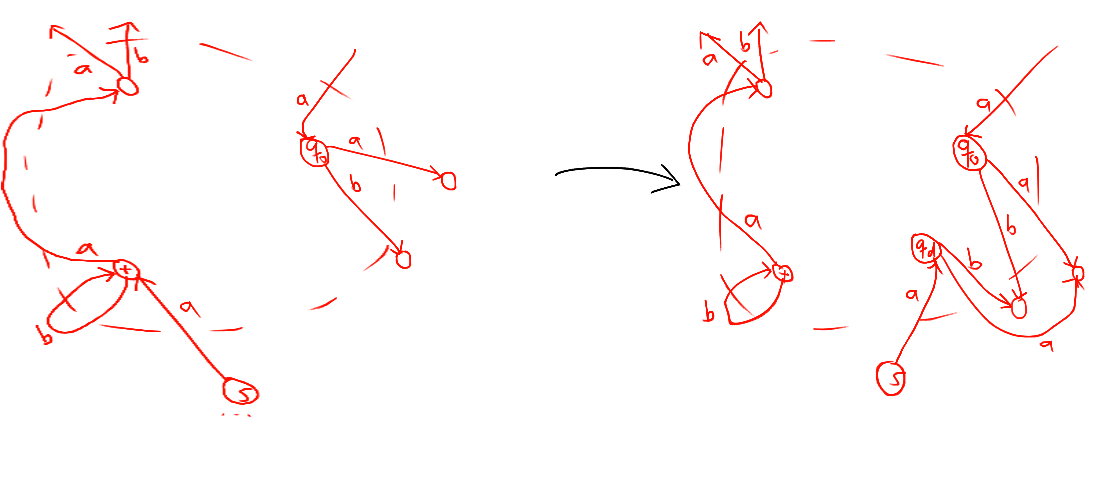
\includegraphics[width=\linewidth]{images/dfa_add_redundant_states.png}
	\caption{If an equivalence class (here denoted by the states in the dashed area) contains a state with 2 or more ingoing transitions (in this case $t$), then a state equivalent to any of the classes states may be added. Here $q_r$ is equivalent to $q_o$ and is ``stealing'' the ingoing transition $\delta(s, a)$ from $t$.}
	\label{fig:dfa_add_redundant_states}
\end{figure}
\gregor{Talk somewhere about eq. automaton and extending it. An eq. class of reach. q's can be max. |$\Sigma$| big. From this can compute the max. number of dupl. states which can be added.}

\subsection{The algorithm}

\vspace{0.2cm}
\begin{spacing}{1}
\begin{algorithmic}[1]
	\Function{AddRedundantStates}{$A, d$}
	\State $K \gets \{\ \{q\}\ |\ q \in Q\ \}$ \Comment{tracks the equivalence classes of $A$}
	\State $k(q) = C$ such that $q \in C$ and $C \in K$ \Comment{returns the equivalence class to $q$}
	\State $in(q) = |d^-(q)|$ for all $q \in Q$ \Comment{tracks the number of ingoing t.}
	
	\For {$d$ \textbf{times}}
		\For {$q$ \textbf{in} $Q$} \Comment{find a duplicatable state $q_o$}
			\If {$in(q) \geq 2$}
				\State $q_0 \gets$ random chosen state from $k(q)$
				\State \textbf{break}
			\EndIf
		\EndFor
		
		\State $q_r \gets$ unused state label \Comment{create to $q_o$ equivalent state $q_r$}
		\State $Q \gets Q \cup \{ q_r \}$
		\State $k(q_o) \gets k(q_o) \cup \{q_r\}$
		
		\For {$\sigma$ \textbf{in} $\Sigma$} \Comment{add $d^+(q_r)$}
			\State $\delta(q_r, \sigma) =$ random chosen state from $k(\delta(q_o, \sigma))$
		\EndFor
		
		\State $P \gets \{\ ((s, \sigma), t) \in \delta\ |\ t \in k(q_o),\ in(t) \geq 2\ \}$ \Comment{add $d^-(q_r)$}
		\State $C \gets$ random nonempty subset of $P$
		\For {$((s, \sigma), t)$ \textbf{in} $C$}
			\State $in(t) \gets in(t) - 1$
			\State $in(q_r) \gets 1$
			\State $t \gets q_r$
		\EndFor
	\EndFor
	\State \Return $A$
	\EndFunction
\end{algorithmic}
\end{spacing}
\vspace{0.2cm}

\subsection{Adding redundant states does not change L}

p. 159 Hopcroft

\subsection{Adding redundant states does not change $\mmD$}

To prove this statement, we will prove two minor propositions first.

\begin{lemma}[Semantics of $(p,q) \in m(n)$] \label{ch:3:semantics-of-m(n)}
	\begin{multline*}
	(p,q) \in m(n) \Longleftrightarrow 
	\exists w\in\Sigma^*\colon |w| = n\ \land \\
	(\delta^*(p,w) \in F \Leftrightarrow \delta^*(q,w) \notin F)
	\end{multline*}
\end{lemma}

\begin{proof}
	See TI-Lecture ch. 4 ``Minimization'' p. 18.
\end{proof}

\begin{lemma}[Semantics of $\mmD(A) = n$] \label{ch:3:semantics-of-D(A)}
	\begin{multline*}
		\mmD(A) =\ n \Rightarrow \\
		n = \max_{n \in \mathbb{N}}\ \ \exists p, q \in Q\ \ \exists w \in \Sigma^* \colon |w| = n - 1\ \land \\
		(\delta^*(p,w) \in F \Leftrightarrow \delta^*(q,w) \notin F)
	\end{multline*}
\end{lemma}

\begin{proof}
	\begin{description}
		\item
		
		Via direct proof.
		
		Assume $m$-\CompDist(A) has done $n$ iterations (so $\mmD(A) = n$). We then know, that
		\begin{itemize}
			\item $\forall i \in [0,n-1]\colon m(i) \neq \emptyset$
			\item $m(n)= \emptyset$
		\end{itemize}
		$m$-\CompDist(A) terminates iff $m(i) = \emptyset$. If the first point would not hold, then the algorithm would have stopped before.
		
		Since the algorithm did $n$ iterations, the internal variable $i$ must be $n$ at the end of the last iteration. The terminating condition is $m(i) \neq \emptyset$; thus follows the second point.
		
		Recall the statement from lemma~\ref{ch:3:semantics-of-m(n)}:
		\begin{multline*}
		(p,q) \in m(n) \Longleftrightarrow 
		\exists w\in\Sigma^*\colon |w| = n\ \land \\
		(\delta^*(p,w) \in F \Leftrightarrow \delta^*(q,w) \notin F)
		\end{multline*}
	
		% a possible word per definition of D(A), m(i) and lemma
		
		Following this lemma and having $m(n-1) \neq \emptyset$ in mind, we can deduce that there exists at least one word $w\in\Sigma^*$ with $|w| = n-1$ such that for two $p,q \in Q\colon (\delta^*(p,w) \in F \land \delta^*(q,w) \notin F)$.
		
		% There is no word longer than that
		
		There cannot be any two states $p',q'\in Q$ and a word $w'\in\Sigma^*$ with $|w'| > n-1$ fulfilling this property. We could write $w'$ as $u'v'$ with $|v'| = n$. Then $m(n)$ would be non-empty, which is contradictory.
	\end{description}
\end{proof}

\begin{theorem}[]
	Adding redundant states to an automaton $A$ does not increase the number of iterations in the \CompDist-algorithm for $A$.
\end{theorem}

\begin{proof}
	\begin{description}
		\item
		
		Proof per contradiction.
		
		Let's assume adding redundant states $q_r^1, \ldots, q_r^n$ to a given automaton $A = (Q, \Sigma, \delta, s, F)$ results in an automaton $A' = (Q', \Sigma, \delta', s, F')$ whereas $\mmD(A) < \mmD(A')$.
		
		Concerning $A'$ we can say the following:
		\begin{itemize}
			\item $Q' = Q \cup \{ q_r^1, \ldots, q_r^n \}$
			%			\item $\delta \subseteq \delta'$
			%			\item $F \subseteq F'$
			\item W.l.o.g. $\exists q_o^1 \in Q \colon \exists q_o^2 \ldots q_o^n \in Q \colon\ \sim_A'(q_o^1, q_r^1), \ldots, \sim_A'(q_o^n, q_r^n)$
		\end{itemize}
		Let us furthermore say that $\mmD(A) = i$ and $\mmD(A') = j$. Recall now lemma~\ref{ch:3:semantics-of-D(A)}:
		\begin{multline*}
		\mmD(A) =\ n \Rightarrow \\
		n = \max_{n \in \mathbb{N}}\ \ \exists p, q \in Q\ \ \exists w \in \Sigma^* \colon |w| = n - 1\ \land \\
		(\delta^*(p,w) \in F \Leftrightarrow \delta^*(q,w) \notin F)
		\end{multline*}
		According to this lemma there must be a pair $s, t \in Q'$ to which exists a word $w \in \Sigma'^*$, $|w| = j - 1$, such that $\delta'^*(s,w) \in F' \Leftrightarrow \delta'^*(t,w) \notin F'$.
		
		Let us split $w$ as $w = uv$ such that $|v| = i$, which is exactly one symbol longer than the longest minimization word of $A$. We can formulate the following statement:
		\begin{equation}
		\text{There must exist }p, q \in Q'\text{ such that }\delta'^*(p,v) \in F' \Leftrightarrow \delta'^*(q,v) \notin F'.
		\end{equation}
		\gregor{hidden formulations here}
		%There must exist $p, q \in Q'$ such that $\delta'^*(p,v) \in F' \Leftrightarrow \delta'^*(q,v) \notin F'$.
		
		%So there exists a minimization word $v$ in $A'$, which is exactly one symbol longer than the longest minimization word of $A$. This word has length $i$ and is detected at minimization depth $i + 1$.
		
		We can therefore state, that $\neg(p \in Q \land q \in Q)$, because else $\mmD(A)$ would be higher than $i$ too.  So at least one of $p,q$ must be in $Q' \setminus Q$ which is exactly $\{ q_r^1, \ldots, q_r^n \}$.
		
		\begin{itemize}
			\item Every $q_r^k$ is $d_{A'}$-equivalent to a $q \in Q$
			\item In every case, $p,q$ can be $d_{A'}$-exchanged s.t. $p,q \in Q$
			\item But that's contradictory to $\mmD(A) = n$, because $p,q$ belong to a minimization word $w = n-1$
		\end{itemize}
		
%		Since $q_r$ is the only new state in $A'$ compared to $A$, we can conclude that at least one of both states must be $q_r$. Since $p = q_r = q$ is contradictory (\gregor{why?}), we can conclude that exactly one of both states $p, q$ is $q_r$ and that the other one is not.
%		
%		W.l.o.g.\ we say $q = q_r$ and $p \in Q' \setminus \{q_r\} = Q$ and reformulate our statement above:
%		\begin{equation}
%		\text{There must exist a }p \in Q\text{ such that }\delta'^*(p,v) \in F' \Leftrightarrow \delta'^*(q_r,v) \notin F'.
%		\end{equation}
%		\gregor{hidden formulations here}
%		
%		%Therefore we know there exists a state $p \in Q$ such that $\exists v \in \Sigma^*$, $|v| = i$ and $\delta'^*(p,v) \in F' \Leftrightarrow \delta'^*(q_r,v) \notin F'$
%		
%		Since for $q_o \in Q$ the relation $d_{A'}(q_o, q_r)$ is given, we know per definition of $d_{A'}$ that $\forall z\in\Sigma'^*\colon \delta'^*(q_o,z) \in F \Leftrightarrow \delta'^*(q_r,z) \in F$.
%		
%		This implies in combination with statement 2.2, that for $p,q_o$ the word $v\in\Sigma'^*$ would fulfill $\delta'^*(p,v) \in F' \Leftrightarrow \delta'^*(q_o,v) \notin F'$ too. But this is contradictory to $p,q \notin Q$.
	\end{description}
\end{proof}

\gregor{Old proof for one $q_r$}
%\begin{proof}
%	\begin{description}
%		\item
%		
%		Proof per contradiction.
%		
%		Let's assume adding a redundant state $q_r$ to a given automaton $A = (Q, \Sigma, \delta, s, F)$ results in an automaton $A' = (Q', \Sigma, \delta', s, F')$ whereas $\mmD(A) < \mmD(A')$.
%		
%		Concerning $A'$ we can say the following:
%		\begin{itemize}
%			\item $Q' = Q \cup \{ q_r \}$
%			%			\item $\delta \subseteq \delta'$
%			%			\item $F \subseteq F'$
%			\item $\exists q_o \in Q \colon\ \sim_A'(q_o, q_r)$
%		\end{itemize}
%		Let us furthermore say that $\mmD(A) = i$ and $\mmD(A') = j$. Recall now lemma~\ref{ch:3:semantics-of-D(A)}:
%		\begin{multline*}
%			\mmD(A) =\ n \Rightarrow \\
%			n = \max_{n \in \mathbb{N}}\ \ \exists p, q \in Q\ \ \exists w \in \Sigma^* \colon |w| = n - 1\ \land \\
%			(\delta^*(p,w) \in F \Leftrightarrow \delta^*(q,w) \notin F)
%		\end{multline*}
%		According to this lemma there must be a pair $s, t \in Q'$ to which exists a word $w \in \Sigma'^*$, $|w| = j - 1$, such that $\delta'^*(s,w) \in F' \Leftrightarrow \delta'^*(t,w) \notin F'$.
%		
%		Let us split $w$ as $w = uv$, whereas $u,v \in\Sigma'^*$ and $|v| = i$, which is exactly one symbol longer than the longest minimization word of $A$. We can formulate the following statement:
%		\begin{equation}
%		\text{There must exist }p, q \in Q'\text{ such that }\delta'^*(p,v) \in F' \Leftrightarrow \delta'^*(q,v) \notin F'.
%		\end{equation}
%		\gregor{hidden formulations here}
%		%There must exist $p, q \in Q'$ such that $\delta'^*(p,v) \in F' \Leftrightarrow \delta'^*(q,v) \notin F'$.
%		
%		%So there exists a minimization word $v$ in $A'$, which is exactly one symbol longer than the longest minimization word of $A$. This word has length $i$ and is detected at minimization depth $i + 1$.
%		
%		We can therefore state, that $\neg(p \in Q \land q \in Q)$, because else $\mmD(A)$ would be higher than $i$ too. 
%		
%		Since $q_r$ is the only new state in $A'$ compared to $A$, we can conclude that at least one of both states must be $q_r$. Since $p = q_r = q$ is contradictory (\gregor{why?}), we can conclude that exactly one of both states $p, q$ is $q_r$ and that the other one is not.
%		
%		W.l.o.g.\ we say $q = q_r$ and $p \in Q' \setminus \{q_r\} = Q$ and reformulate our statement above:
%		\begin{equation}
%		\text{There must exist a }p \in Q\text{ such that }\delta'^*(p,v) \in F' \Leftrightarrow \delta'^*(q_r,v) \notin F'.
%		\end{equation}
%		\gregor{hidden formulations here}
%		
%		%Therefore we know there exists a state $p \in Q$ such that $\exists v \in \Sigma^*$, $|v| = i$ and $\delta'^*(p,v) \in F' \Leftrightarrow \delta'^*(q_r,v) \notin F'$
%		
%		Since for $q_o \in Q$ the relation $d_{A'}(q_o, q_r)$ is given, we know per definition of $d_{A'}$ that $\forall z\in\Sigma'^*\colon \delta'^*(q_o,z) \in F \Leftrightarrow \delta'^*(q_r,z) \in F$.
%		
%		This implies in combination with statement 2.2, that for $p,q_o$ the word $v\in\Sigma'^*$ would fulfill $\delta'^*(p,v) \in F' \Leftrightarrow \delta'^*(q_o,v) \notin F'$ too. But this is contradictory to $p,q \notin Q$.
%		
%		\gregor{hidden lemma here}
%		
%		%		\begin{lemma}
%		%			\begin{multline*}
%		%				\mmD(A) =\ n \Leftrightarrow \\
%		%				n = \max_{n \in \mathbb{N}}\ \ \exists p, q \in Q\ \ \exists w \in \Sigma^* \colon \\
%		%				|w| = n - 1 \land (\delta^*(p,w) \in F \Leftrightarrow \delta^*(q,w) \notin F)
%		%			\end{multline*}
%		%		\end{lemma}
%	\end{description}
%\end{proof}

\section{Adding unreachable states}

From step 1 of the minimization algorithm we can deduce how to add unreachable states. These can easily be added to a DFA by adding non-start states with no ingoing transitions (see def.~\ref{ch:1:unreachable-states}). Number and nature of outgoing transitions may be arbitrary.

\vspace{0.2cm}
\begin{algorithmic}[1]
	\Function{AddUnreachableStates\ }{$A, u$}
	\For {$u$ \textbf{times}}
		\State $q \gets \max Q + 1$
		\State $Q \gets Q \cup \{ q \}$
		\State $R \gets$ random chosen sample of $|\Sigma|$ states from $Q \setminus \{q\}$
		\For {$\sigma$ \textbf{in} $\Sigma$}
			\State $q' \in R$
			\State $R \gets R \setminus \{q'\}$
			\State $\delta \gets \delta \cup \{ ((q, \sigma), q') \}$
		\EndFor
	\EndFor
	\State \Return $A$
	\EndFunction
\end{algorithmic}
\vspace{0.2cm}

\noindent We have to ensure, that this algorithm does not induce changes in the language.
\begin{lemma}
	Adding unreachable states to a DFA does not change its language.
\end{lemma}
\begin{proof}
	Remember that the language of a DFA $A = (Q, \Sigma, \delta, s, F)$ is defined as $L(A) = \{\ w\ |\ w \in \Sigma^* \ \}$. For any unreachable state $q$ there exists no word $v \in \Sigma^*$ such that $\delta^*(s,v) = q$. Thus such a state cannot be the cause for any word to be in $L(A)$.
\end{proof}

\noindent The question whether adding unreachable states to a DFA changes $\mmD$-value is irrelevant. This is because in the context of the minimization algorithm, unreachable states are eliminated before the \CompDist-algorithm is applied on the task DFA.
